\documentclass{beamer}

\mode<presentation> {

% The Beamer class comes with a number of default slide themes
% which change the colors and layouts of slides. Below this is a list
% of all the themes, uncomment each in turn to see what they look like.

%\usetheme{default}
%\usetheme{AnnArbor}
%\usetheme{Antibes}
%\usetheme{Bergen}
%\usetheme{Berkeley}
%\usetheme{Berlin}
%\usetheme{Boadilla}
%\usetheme{CambridgeUS}
%\usetheme{Copenhagen}
%\usetheme{Darmstadt}
%\usetheme{Dresden}
\usetheme{Frankfurt}
%\usetheme{Goettingen}
%\usetheme{Hannover}
%\usetheme{Ilmenau}
%\usetheme{JuanLesPins}
%\usetheme{Luebeck}
%\usetheme{Madrid}
%\usetheme{Malmoe}
%\usetheme{Marburg}
%\usetheme{Montpellier}
%\usetheme{PaloAlto}
%\usetheme{Pittsburgh}
%\usetheme{Rochester}
%\usetheme{Singapore}
%\usetheme{Szeged}
%\usetheme{Warsaw}

% As well as themes, the Beamer class has a number of color themes
% for any slide theme. Uncomment each of these in turn to see how it
% changes the colors of your current slide theme.

%\usecolortheme{albatross}
%\usecolortheme{beaver}
%\usecolortheme{beetle}
\usecolortheme{crane}
%\usecolortheme{dolphin}
%\usecolortheme{dove}
%\usecolortheme{fly}
%\usecolortheme{lily}
%\usecolortheme{orchid}
%\usecolortheme{rose}
%\usecolortheme{seagull}
%\usecolortheme{seahorse}
%\usecolortheme{whale}
%\usecolortheme{wolverine}

%\setbeamertemplate{footline} % To remove the footer line in all slides uncomment this line
%\setbeamertemplate{footline}[page number] % To replace the footer line in all slides with a simple slide count uncomment this line

%\setbeamertemplate{navigation symbols}{} % To remove the navigation symbols from the bottom of all slides uncomment this line
}

\usepackage{units}
\usepackage{extpfeil}
\usepackage{extarrows} %Allows long equation signs
\usepackage{graphicx} % Allows including images
\usepackage{booktabs} % Allows the use of \toprule, \midrule and \bottomrule in tables
\usepackage{physics}
\usepackage{tikz}
\usepackage{cite}
%花体字母
\usepackage{amsthm,amsmath,amssymb}
\usepackage{mathrsfs}
\usepackage{dutchcal}
\usepackage{circuitikz}
\usepackage{eqnarray}

%----------------------------------------------------------------------------------------
%	TITLE PAGE
%----------------------------------------------------------------------------------------

\title[VP260 RC]{VP260 Recitation Class 5} % The short title appears at the bottom of every slide, the full title is only on the title page

\author{Yanjun Chen} % Your name
\institute[UM-SJTU JI] % Your institution as it will appear on the bottom of every slide, may be shorthand to save space
{
    University of Michigan - Shanghai Jiao Tong University Joint Institute\\% Your institution for the title page
\medskip
}
\date{\today} % Date, can be changed to a custom date

\begin{document}

\begin{frame}
    \titlepage % Print the title page as the first slide
\end{frame}

%----------------------------------------------------------------------------------------
%	 SECTION homework
%----------------------------------------------------------------------------------------

\section{Midterm Exam}

\begin{frame}{Midterm}
    \begin{itemize}
        \item Concepts, definitions.
        \item Qualitatively vs. Quantitatively
    \end{itemize}
\end{frame}


%----------------------------------------------------------------------------------------
%	 SECTION 1
%----------------------------------------------------------------------------------------

\section{Fundamental Concepts} % Section title slide, unnumbered

% \begin{frame}{Backup Materials}
%     \begin{itemize}
%         \item Electrostatics: stationary charges $\Rightarrow$ constant electric field 
%         \item Magnetostatics: steady currents $\Rightarrow$ constant magnetic field 
%     \end{itemize}    

%     \begin{beamerboxesrounded}[shadow=true]{\bf Reynolds Transport Theorem}
%         \begin{equation}
%             \dv{t} \int_{\Omega} F(\va*{x},t) \dd{\tau} = \int_{\Omega} \pdv{F}{t} \dd{\tau} + \oint_{\Sigma} F\va*{v} \vdot \dd{\va{a}}
%         \end{equation}
%         where $\dv{t}$ represents the material (total) derivative.
%     \end{beamerboxesrounded}
%     \vspace{.5em}
%     \begin{beamerboxesrounded}[shadow=true]{\bf Continuity Equation}
%         \begin{equation}
%             \div{\va*{J}} + \pdv{\rho}{t} = 0 
%         \end{equation}
%         where $\va*{J} = \rho \va*{v}$.
%     \end{beamerboxesrounded}

% \end{frame}

\begin{frame}{Law of Biot and Savart}
    \begin{block}{Steady current}
        \begin{equation}
            \pdv{\va{J}}{t} = 0
        \end{equation}
    \end{block}

    \begin{itemize}
        \item Magnetostatics : steady currents produce the magnetic fields that are constant in time.
    \end{itemize}
    

    \begin{beamerboxesrounded}{Law of Biot and Savart}
        \begin{equation}
            \va*{B}(\va*{r}) = \frac{\mu_0}{4\pi} \int_{\varGamma} \frac{I \dd{\va{L}} }{\abs*{\va*{r}-\va*{r'}}^2} \times \frac{\va*{r}-\va*{r'}}{\abs*{\va*{r}-\va*{r'}}}
        \end{equation}      
        \begin{itemize}
            \item $\mu_0=\unit{4\pi\times 10^{-7}}{N/A^2}$.
            \item Speed of light in vacuum: $c^2 = 1/ \epsilon_0 \mu_0$.
        \end{itemize}
    \end{beamerboxesrounded}
\end{frame}



\begin{frame}{Magnetic Field:Examples}
    \begin{block}{Straight current}
        \begin{equation}
            B = \frac{\mu_0 I}{2 \pi r}
        \end{equation}
    \end{block}
    \vfill
    Two wires carrying current: 
        \begin{itemize}
            \item Same direction $\Rightarrow$ attraction 
            \item Opposite directions $\Rightarrow$ repulsion
        \end{itemize}
\end{frame}


\begin{frame}{Magnetic Field:Examples}
    \begin{beamerboxesrounded}{Circular current loop}
        \begin{equation}
            B = \frac{N\mu_0I}{2} \frac{R^2}{(z^2+R^2)^{3/2}}
        \end{equation}
    \end{beamerboxesrounded}
    \vfill
    \begin{figure}[htbp]
        \centering
        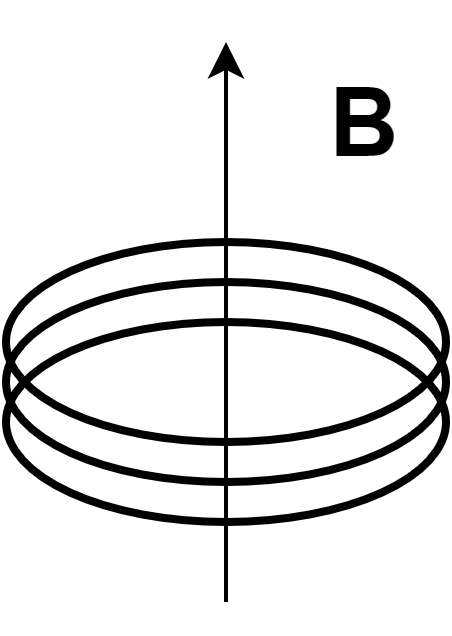
\includegraphics[scale=0.8]{images/loop.png}
    \end{figure}
\end{frame}


\begin{frame}{Ampere's Law}
    \begin{figure}[htbp]
        \centering
        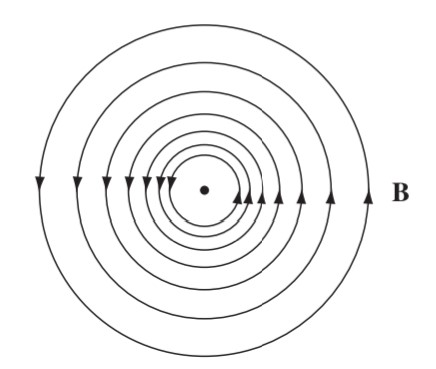
\includegraphics[width=0.3\textwidth]{Images/amp.jpg}
    \end{figure}
    For any closed loop,
    \begin{equation}
        \oint \va{B} \vdot \dd{\va{l}} = \oint \frac{\mu_0 I}{2 \pi s} \dd{l} = \mu_0 I.
    \end{equation}

    Hence,
    \begin{equation}
        \oint \va{B} \vdot \dd{\va{l}} = \mu_0 I_{\text{enc}} = \mu_0 \int \va{J} \vdot \dd{\va{a}}
    \end{equation}
\end{frame}


\begin{frame}{Ampere's Law}
    \begin{block}{Ampere's law}
        \begin{equation}
            \curl{\va*{B}} = \mu_0 \va*{J}
        \end{equation}
        \begin{equation}
            \oint \va*{B} \vdot \dd{\va*{l}} = \mu_0 I_{\text{enc}} 
        \end{equation}
    \end{block}
\end{frame}

\begin{frame}{Comparison Between $\va{E}$ and $\va{B}$}
    \begin{itemize}
        \item Electrostatics:
        \begin{equation}
            \pdv{\rho}{t} = 0
        \end{equation}
        \item Magnetostatics:
        \begin{equation}
            \pdv{\va{J}}{t} = 0
        \end{equation}
    \end{itemize}
    \begin{table}[htbp]
        \centering
        \begin{tabular}{lcc}
            \toprule
            Field & Integral Form & Differential Form \\
            \midrule
            Electrostatics & $\oint \va{E}\vdot\dd{\va{a}}=\frac{Q_encl}{\epsilon_0}$ & $\div{\va{E}} = \frac{\rho}{\epsilon_0}$ \\ \addlinespace
                           & $\oint \va{E}\vdot\dd{\va{l}}=0$ & $\curl{\va{E}}=\va{0}$ \\ \addlinespace
            Magnetostatics & $\oint \va{B}\vdot\dd{\va{a}}=0$ & $\div{\va{B}} = 0$ \\ \addlinespace
                           & $\oint \va{B}\vdot\dd{\va{l}}=\mu_0 I_{encl}$ & $\curl{\va{B}}=\mu_0 \va{J}$ \\
            \bottomrule
        \end{tabular}
    \end{table}
\end{frame}

%----------------------------------------------------------------------------------------
%	 Section 2
%----------------------------------------------------------------------------------------

\section{Exercise}

\begin{frame}{Exercise 1}
    A conductor shaped as shown in the figure carries constant current $I$. Find the magnetic field at the center of the circle.
    \vspace{1em}
    \begin{figure}[htbp]
        \centering
        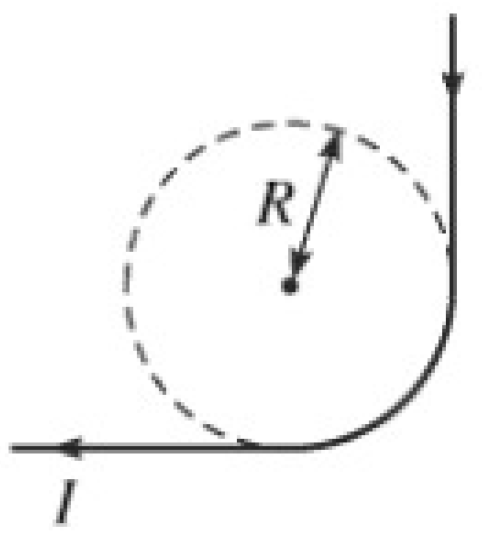
\includegraphics[scale=0.4]{images/e1.png}
    \end{figure}
\end{frame}

\begin{frame}{Exercise 2}
    A conical surface ($x^2 + y^2 = z^2, 0 \le z \le h$) charged uniformly with surface density of charge $\sigma$ rotates about it axis of symmetry with constant angular velocity $\omega$. Find the magnetic field in the origin.
\end{frame}

\begin{frame}{Exercise 3}
    Suppose you have two infinite straight line charges $\lambda$, a distance $d$ apart, moving along at a constant speed $v$. How great would $v$ have to be in order for the magnetic attraction to balance the electrical repulsion? Is this a reasonable sort of speed?.
    \vspace{1em}
    \begin{figure}[htbp]
        \centering
        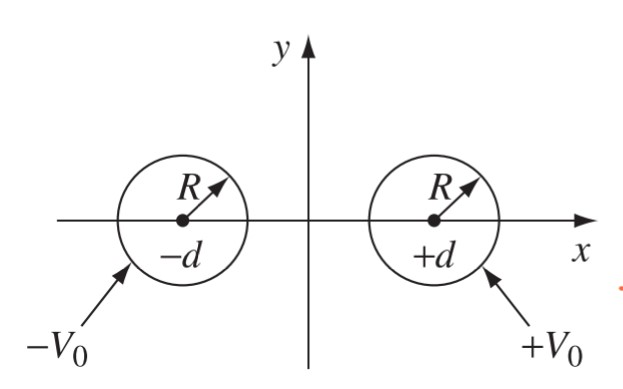
\includegraphics[scale=0.8]{images/e3.jpg}
        \label{Fig:}
    \end{figure}
\end{frame}

%----------------------------------------------------------------------------------------
%	 CLOSING/SUPPLEMENTARY SLIDES
%----------------------------------------------------------------------------------------
\section{Appendix}


\begin{frame}
    \begin{center}
        \LARGE\bf Thanks for listening!
    \end{center}
\end{frame}


%----------------------------------------------------------------------------------------

\begin{frame}{\bf References}
	\nocite{*} % Display all references regardless of if they were cited
	\bibliography{example.bib}
	\bibliographystyle{plain}
\end{frame}

\end{document}

